\chapter{Data}
    
\section{Description of Data}
    As explained in Chapter 1 the data that will be used is provided by the Center for Molecular Imaging and are MRI rat brain images over time. 
    The MR images themselves vary between each different rat, but also as seen can vary significantly in each group.
\subsection{Brain Regions}
    The brain regions that we will segment are shown in in figure ~\ref{fig:segmentation regions}. 
    There are 7 total regions listed in the image. 
    One additional region that is segmented that is not in the figure is the cerebellum. 
    Each region will also be separated in to a left and a right side region of the brain except for the medial thalamus. 
    This means that in total our model will segment 14 different regions. 
    Each of these regions are very different where we have some that are quite close to each other, the inner and outer cerebral cortex layers, and others that are all alone, the piriform cortex. 
    There are also very small regions like the medial thalamus and very large regions like the cerebellum to take into account. 
    


    

\subsection{Image Pre-processing}
    Before the rat brain MR images can be used in the model they need to be pre-processed to facilitate training. 
    The rat brain MRI images are taken as nifty files. 
    An example of an unprocessed MR image vs the processed MR image is shown in figure ~\ref{fig:procvsUnproccMRI}.
    The processed image is larger and better contrasted than the pre-processed image, which will help the model train faster.
    We will talk about the exact pre-processing technique as applied to the rat brain MR images.
    
\begin{figure}
\centering
\begin{subfigure}{.5\textwidth}
  \centering
  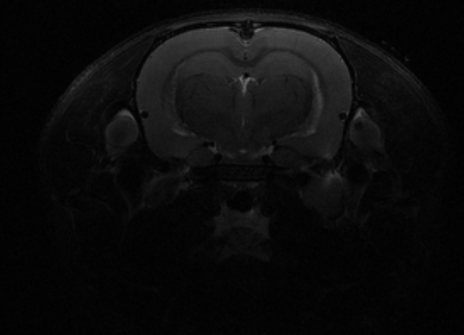
\includegraphics[width=0.9\linewidth]{MRI_veh01.png}
  \caption{Unprocessed T2w MR image }
  \label{fig:unprocessedMRI}
\end{subfigure}%
\begin{subfigure}{.5\textwidth}
  \centering
  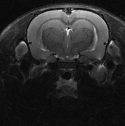
\includegraphics[width=0.8\linewidth]{post_MRI_veh01.png}
  \caption{Pre-processed T2w MR image}
  \label{fig:processedMRI}
\end{subfigure}
\caption{This figure shows the image pre-processing technique as applied to the rat brain MR images.}
\label{fig:procvsUnproccMRI}
\end{figure}

\subsubsection{Normalization and Cropping}
    One of the first pre-processing step is center cropping. 
    As shown in the unprocessed MRI image the rat brain is covered with a lot of background pixels unneeded for the model.
    In order to make the model more efficient the images are center cropped and downsampled from 280x200x44 to 128x128x44.
    This helps to emphasize the more important regions and leave out the areas that are not useful for the model. 
    We also downsample the images to 128x128 in order to be able to have enough memory for the gpu to be able to train the model.
    
    The images are then normalized in order to keep the range of the images the same and decrease the bias in the model. 
    They are normalized by dividing by the max pixel value per MRI volume or 128x128x44 image.


\subsubsection{Biased MRI images}
     One very important processing technique used for MR images is that they need to be corrected for the bias field signal. 
     This signal is produced when taking the MRI images and causes a fluctuation in the gray values in the MRI image. 
     This can be corrected for by estimating the bias field signal using a surface fitting approach \cite{Juntu2005BiasFC}. 
     As seen in figure ~\ref{fig:biasedvscorrMRI}, the fluctuations caused by the bias signal can be very large and greatly affect the performance of the model. 
    
\begin{figure}
\centering
\begin{subfigure}{.5\textwidth}
  \centering
  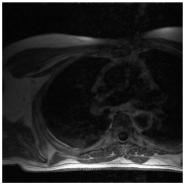
\includegraphics[width=.6\linewidth]{baisedMRIimage.png}
  \caption{Example of a biased MRI image due to the bias field signal}
  \label{fig:baisedMRI}
\end{subfigure}%
\begin{subfigure}{.5\textwidth}
  \centering
  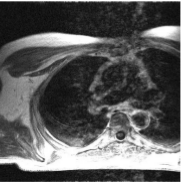
\includegraphics[width=.6\linewidth]{CorrectedMRIBias.png}
  \caption{The same image but corrected for the bias field signal using the surface fitting approach}
  \label{fig:correctedMRI}
\end{subfigure}
\caption{This figure shows some the effect of bias field signal on MRI images. }
\label{fig:biasedvscorrMRI}
\end{figure}
    

\subsection{Data Augmentation}
    Data augmentation is very useful in machine learning tasks. 
    One of the main ways to have a model generalize better is to train the model on a more diverse dataset. 
    Data augmentation takes advantage of basic image transforms to "create" new images for the model to train on \cite{articledataAug}. 
    Some examples of basic data augmentation transforms are scale, crop, brightness, rotation, flipping, padding, etc. 
    All of these basic transforms when applied to an image will change the image and when put through the model will allow it to be more robust. 
    Many papers utilize data augmentation in order to increase the robustness and precision of their model ~\cite{NIPS2012_Krizhevsky}, ~\cite{articledataAug}, ~\cite{DBLP:journals/corr/MilletariNA16}, ~\cite{DBLP:journals/corr/RonnebergerFB15}.
    Other papers though report that data augmentation did not improve their results significantly or did not use data augmentation ~\cite{DBLP:journals/corr/HavaeiDWBCBPJL15}, ~\cite{DBLP:journals/corr/abs-1805-10720}. 
    When it comes to data augmentation for medical images, the methods that do utilize data augmentation only use a certain amount of transformations ~\cite{10.1007/978-3-030-01449-0_16dilatedunet}. 
    The reason behind this is that medical images are usually taken in a controlled environment where the patient lays on a bed and is told not to move. 
    For this reason, in this thesis we only adopt a rotation of 10 degrees, horizontal flip, image shift of 20\%, and a brightness range from 70\% to 100\%.
    We implement a small rotation as well as well as a small image shift and horizontal flip because not all images are taken perfectly in the same area every time even though it is a controlled environment. 
    A brightness range is also implemented because depending on the imaging condition the tissue will be brighter or darker compared to the surrounding tissue. 
    Some examples of the data augmented images are shown in figure ~\ref{fig:dataAugImage}. 
    

\begin{figure}[ht] 
  \begin{minipage}[b]{0.5\linewidth}
    \centering
    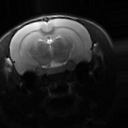
\includegraphics[width=\linewidth]{0.png} 
  \end{minipage} 
  \begin{minipage}[b]{0.5\linewidth}
    \centering
    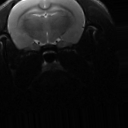
\includegraphics[width=\linewidth]{1.png} 
  \end{minipage} 
  \begin{minipage}[b]{0.5\linewidth}
    \centering
    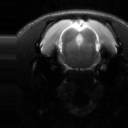
\includegraphics[width=\linewidth]{3.png} 
  \end{minipage}
  \hfill
  \begin{minipage}[b]{0.5\linewidth}
    \centering
    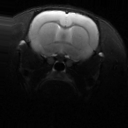
\includegraphics[width=\linewidth]{9.png} 
  \end{minipage} 
  \caption{Some examples of the data augmented MRI images. }
  \label{fig:dataAugImage} 
\end{figure}

\subsection{Image Data}
    As explained before a total of 40 rats were imaged with a total of 120 MRI images taken. 
    Due to some problems with imaging only 115 animal scans were available for use within the model. 
    The data was split between a training set, a validation set, and test set to prevent overfitting in our model. 
    Since the data is also split between 4 different animal groups the validation and test dataset has one animal from each group to see how each group performs from the model. 
   Each animal has MR images at three different time points as well and so the validation/test sets consist of 12 different animal MR images while the training dataset consists of 103 animal MR images. 
    Data augmentation was also utilized as explained before and the dataset was doubled and data augmentation applied to the replicated data. 
    The training dataset consists of a total of 206 MR images each of size 128x128x44 or 9,064 total 2D 1MR images while the validation and test sets consists of 12 MR images each of size 128x128xx44 or 528 2D MR images. 